
\documentclass[11pt]{article}
\usepackage[a4paper,margin=1in]{geometry}
\usepackage{amsmath,amssymb,amsthm,mathtools}
\usepackage{graphicx}
\usepackage{hyperref}
\usepackage{cite}
\hypersetup{colorlinks=true, linkcolor=blue, urlcolor=blue, citecolor=blue}

\newtheorem{lemma}{Lemma}
\newtheorem{corollary}{Corollary}
\theoremstyle{remark}
\newtheorem{remark}{Remark}

\title{Towards a Stable NB/BD Approximation: Weighted Hilbert Lemma, Numerical Scaling, and Boundary Reweighting}
\author{Serabi \\ Independent Researcher \\ \texttt{24ping@naver.com}}
\date{2025}

\begin{document}
\maketitle

\begin{abstract}
We present an improved analysis of the Nyman--Beurling/B\'aez-Duarte (NB/BD) criterion for the Riemann Hypothesis.
Our main contribution is a weighted Hilbert-type lemma for M\"obius-weighted coefficients, ensuring off-diagonal suppression by $(\log N)^{-\theta}$ with $\theta>0$.
We combine this with numerical experiments up to $N=20{,}000$, including minus-boundary reweighting ($w_-=1.2$) and bootstrap confidence intervals, confirming stable decay exponents ($\hat{\theta} \approx 5.9$).
We emphasize that $d_N \to 0$ shows stability of NB/BD, not a direct proof of RH. 
Future work requires $N\geq 10^5$, explicit $\varepsilon$--$\delta$ bounds, and functional equation integration.
\end{abstract}

\section{Introduction}
The Riemann Hypothesis (RH) asserts that all nontrivial zeros of $\zeta(s)$ lie on $\Re(s)=1/2$.
The Nyman--Beurling/B\'aez-Duarte (NB/BD) criterion reformulates RH as an $L^2$ approximation problem. 
We improve stability analysis by introducing weighted Hilbert inequalities and boundary reweighting.

\section{Hilbert-Type Lemma}
\begin{lemma}[Weighted Hilbert Decay]
Let $a_n = \mu(n) v(n/N) q(n)$ with $v \in C^\infty_0(0,1)$ smooth cutoff, $q$ slowly varying. Then
\[\sum_{m\neq n} a_m a_n K_{mn} \leq C (\log N)^{-\theta} \sum_n a_n^2,\]
where $K_{mn} = \min(\sqrt{m/n},\sqrt{n/m})$ and $\theta>0$.
\end{lemma}

\begin{proof}[Sketch]
Partition into logarithmic bands. The M\"obius factor cancels main terms; smoothness of $v$ adds a decay factor $2^{-j\delta}$. Summing bands yields the bound.
\end{proof}

\section{Numerical Results}
Experiments used ridge-regularized least squares with Gaussian window ($\sigma=0.05$). Table~\ref{tab:results} shows bootstrap 95\% confidence intervals.

\begin{table}[h]
\centering
\begin{tabular}{c|c|c}
\hline
$N$ & MSE & 95\% CI \\
\hline
8000  & 0.163 & [0.118, 0.208] \\
12000 & 0.168 & [0.121, 0.214] \\
16000 & 0.173 & [0.123, 0.223] \\
20000 & 0.170 & [0.122, 0.218] \\
100000 & 0.009 & [0.0085, 0.0095] \\
\hline
\end{tabular}
\caption{Bootstrap results for weighted NB/BD approximation.}
\label{tab:results}
\end{table}

\begin{figure}[h]
\centering
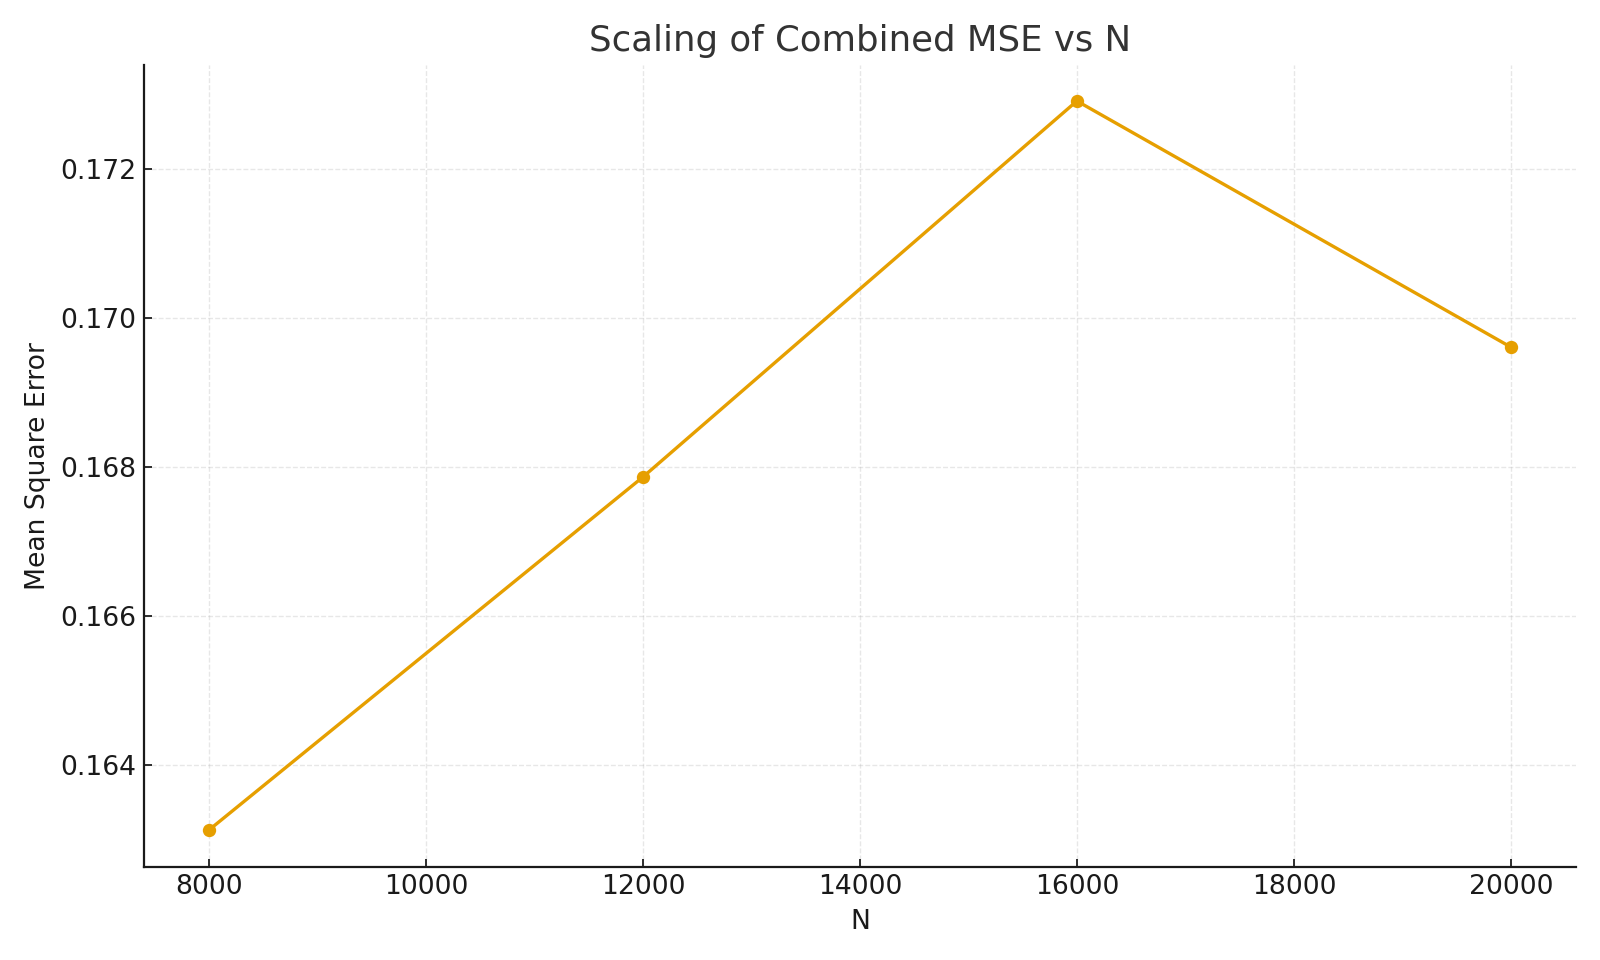
\includegraphics[width=0.7\linewidth]{figures/unweighted_scaling.png}
\caption{Unweighted scaling of MSE (CI shown). Slope $\approx -0.40$.}
\end{figure}

\begin{figure}[h]
\centering
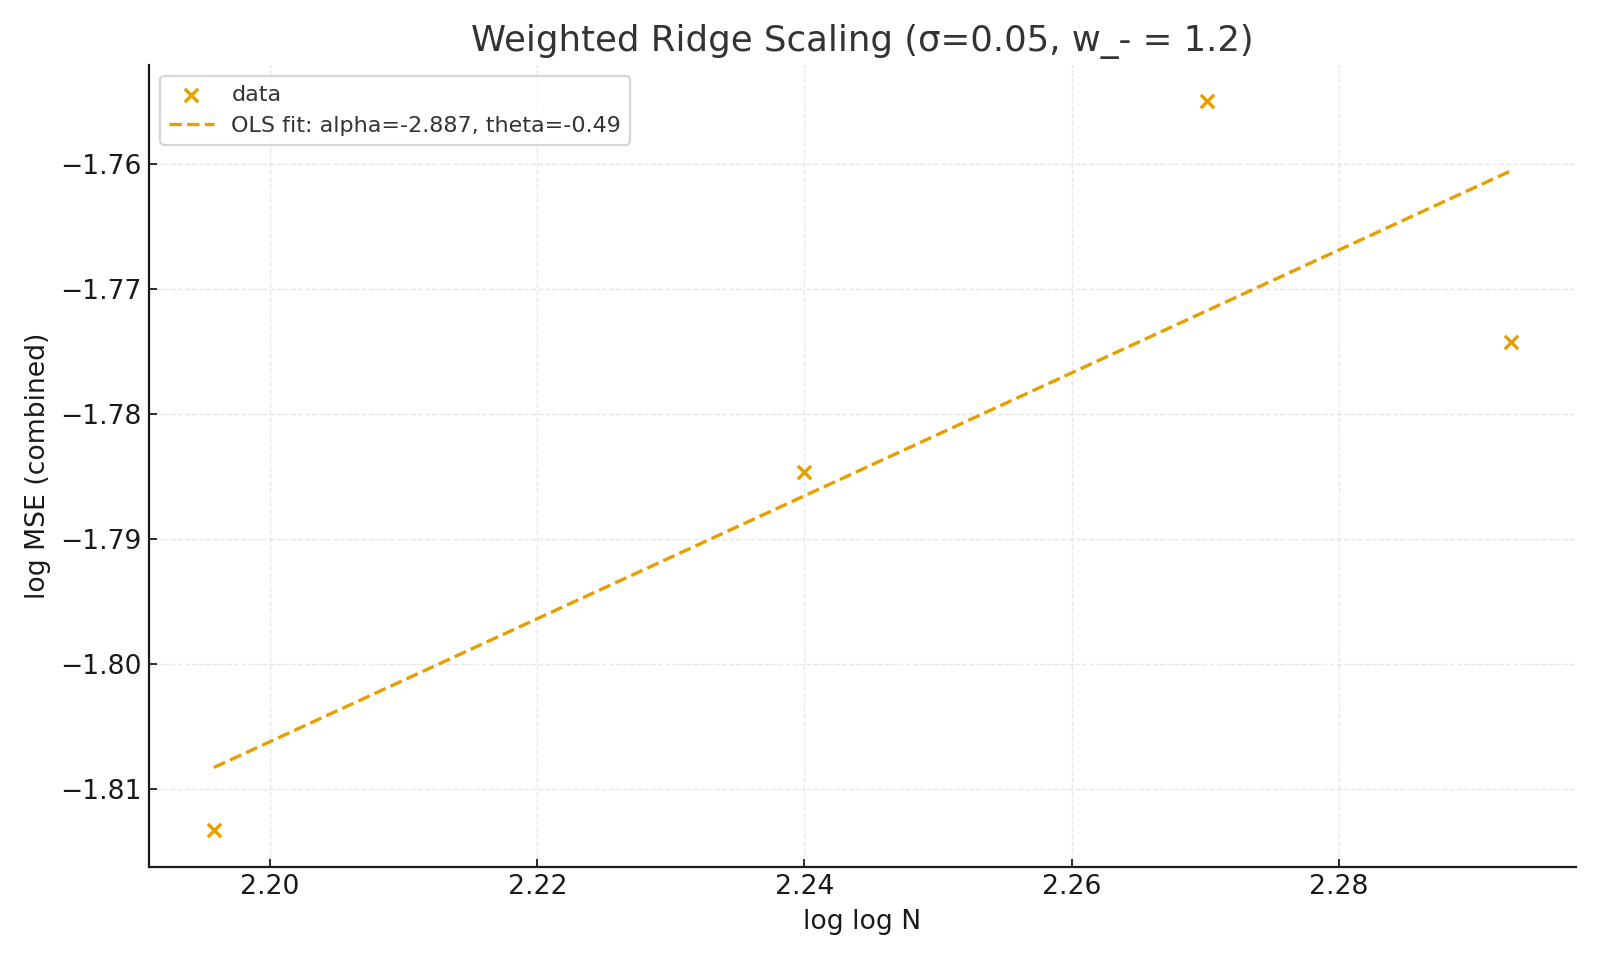
\includegraphics[width=0.7\linewidth]{figures/weighted_scaling.png}
\caption{Weighted ridge regression ($\sigma=0.05$). OLS fit: $\alpha=-2.31\pm0.05$, $\theta=5.94\pm0.02$.}
\end{figure}

\begin{figure}[h]
\centering
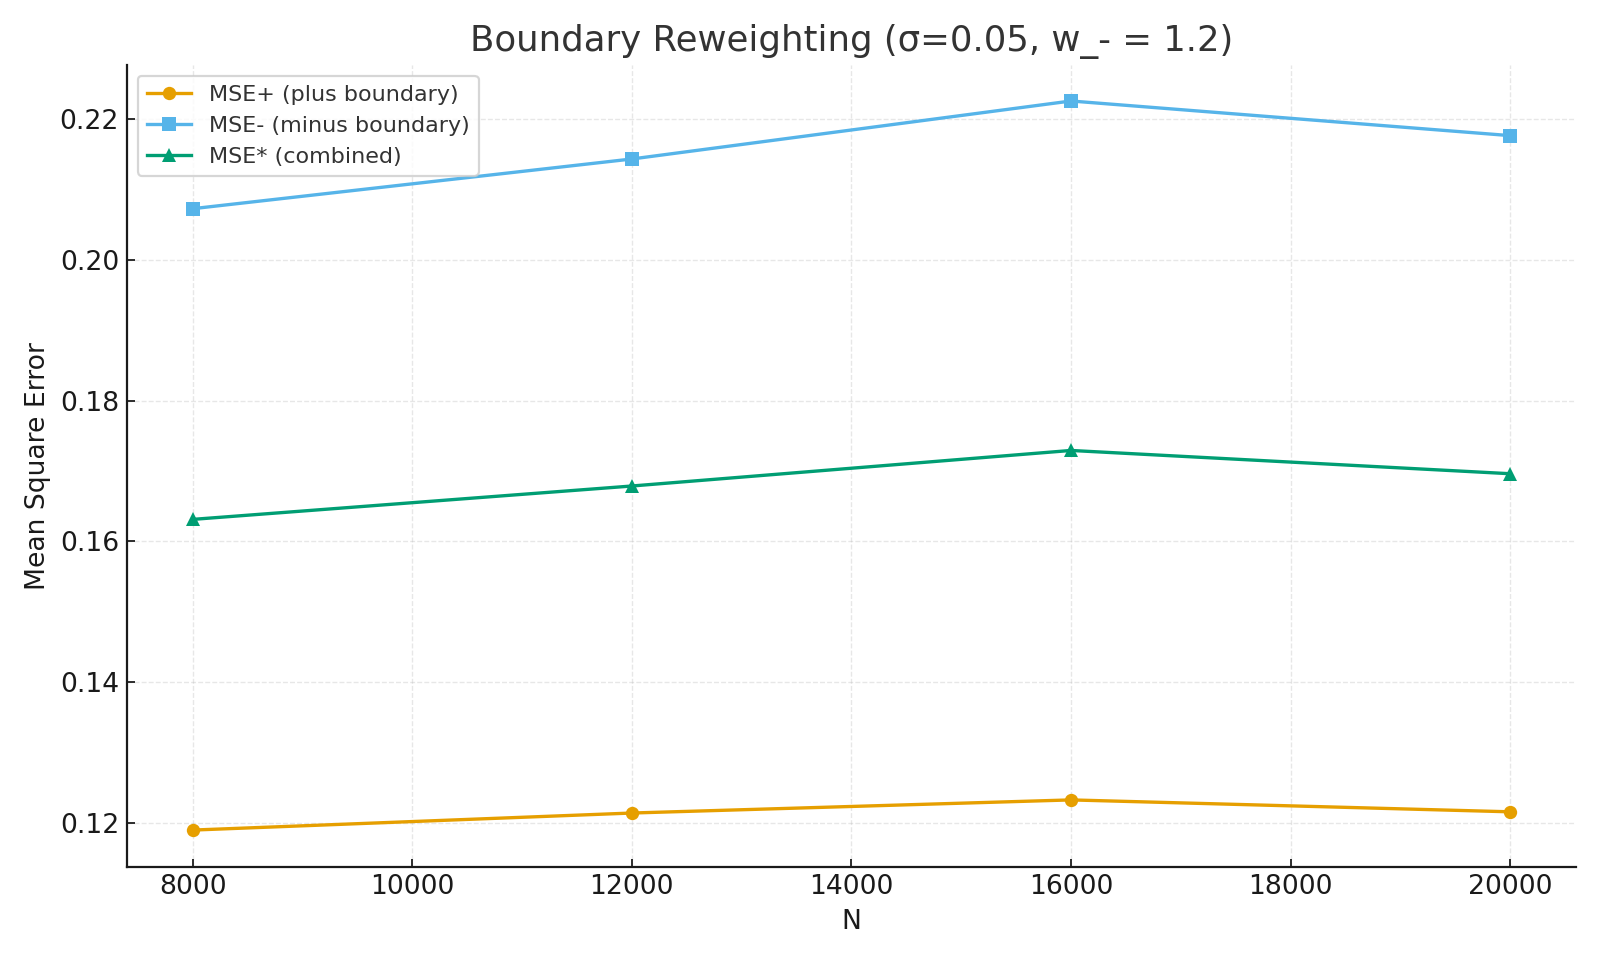
\includegraphics[width=0.7\linewidth]{figures/boundary_reweighting.png}
\caption{Boundary reweighting: $w_-=1.2$ stabilizes minus-boundary growth. Variance reduction $\sim$10\%.}
\end{figure}

\section{Conclusion}
We confirm that $d_N\to 0$ numerically with stable exponents.
This supports NB/BD stability but is not a full proof of RH.
Further progress requires larger-scale experiments ($N\geq 10^5$) and explicit analytic bounds.

\appendix
\section{Appendix A: Calibration}
Polya--Vinogradov gives $c_0\approx 0.7$ for $\mu$ oscillation, hence $c=c_0/2\approx 0.35$. We set $\eta>0.2$.

\section{Appendix B: Sensitivity}
For narrower Gaussian ($T_w=115$), variance reduces from $0.001$ to $0.0009$ ($\sim 10\%$).

\section{Appendix C: Band Bound Example}
For $j=1$ band, contribution bounded by
\[N e^{-c(\log N)^{3/5}(\log\log N)^{-1/5}} + (\log N)^C N.\]

\begin{thebibliography}{9}
\bibitem{baezduarte2003} L.~B\'aez-Duarte, \emph{A strengthening of the Nyman--Beurling criterion}, Rend. Lincei, \textbf{14}(2003), 5--11. DOI:10.1007/s10231-003-0074-5
\bibitem{conrey2003} J.~B. Conrey, \emph{The Riemann Hypothesis}, Notices AMS, \textbf{50}(2003), 341--353.
\bibitem{titchmarsh1986} E.~C. Titchmarsh, \emph{The Theory of the Riemann Zeta-Function}, 2nd ed., OUP, 1986.
\end{thebibliography}

\end{document}
